\newcommand{\nevents}{8453} %% BUT HARDCODED ELSEWHERE

\chapter{Analysis Method}
\label{anMeth}
%I guess this is the part of the analysis that's not included in event selection.  
%SO, how to get the cross section, like the main formula, 
%and where all the numbers came from (especially the ones we haven't calculated yet).

The previous chapter explained how the data events used 
in the analysis were selected.  
The endpoint of that chapter was a set of 
\Zee candidate events: 
events that had two well-reconstructed electrons 
with an invariant mass between 60 and 120 GeV.  % NEED TO EXPLAIN INV MASS BEFORE THIS
This chapter explains the rest of the process 
needed to obtain the result, the final cross section.  
This includes assembling all the necessary components % SECTION TITLE! referring to assembling the components
of the calculation, 
as well as determining the uncertainty 
inherent in each component 
and combining the uncertainties into one overall value.  

%recap of invariant mass?

\section{Invariant Mass Spectrum} % DON'T REALLY NEED ALL EXPLANATORY STUFF HERE, IF IN INTRO CH???
\label{anMeth:invmass}
As explained in Section~\ref{theory:Zprod}, % it's done in introductory material
the invariant mass of a set of decay-product particles is 
%CONCEPTUAL EXPLANATION.
essentially the mass of the original particle that decayed. 
%to form the end-products.  
It is defined mathematically by %as 
\[
M_{inv}^2 = \left( \sum E \right)^2 - \left\| \sum \mathbf{p} \right\|^2
\]
where $ \mathbf{p} $ is the momentum 
and $ E $ the energy for a given particle; 
$ \sum $ denotes the sum over all particles 
-- a vector sum in the case of momentum, 
while $\left\| \mathbf{p} \right\|$ denotes the momentum's magnitude.  
In our case, for a two-particle system, this can be written as 
\[
M_{inv} = \sqrt{ \left(E_1 + E_2\right)^2 - \left\|\mathbf{p}_1 + \mathbf{p}_2\right\|^2 }
\]
The invariant mass distribution within the mass window 
for the electron pairs 
in the events surviving all selection cuts is shown in 
Fig.~\ref{fig:InvMass}.  
An explanation of how the different simulation 
samples were combined can be 
found in Section FIXME.  
The peak around the Z mass (91 GeV) is clearly visible 
in both the Monte Carlo (solid) and data (points) distributions.  
The background contributions estimated from Monte Carlo simulation 
are shown as the colored (grayscale) areas.  
A slight shift in the peak position along the x-axis is 
evident, due to slight miscalibrations of 
the calorimeter response to given energies.  
This difference is accounted for in the 
systematic uncertainty due to the electron energy scale 
(see Section~\ref{anMeth:SystsOtherEleEScale}).  
The selected events are also divided into categories according 
to which part of the detector, barrel or endcap, 
each of their electron legs were located, 
and the resulting invariant mass spectra are 
shown in Fig.~\ref{fig:InvMassEtaDiv}.  
Agreement in each case is good to within the 
uncertainty.  

%ALSO TALK ABOUT HOW PLOTS SCALED??!!  
%somewhere, like in event selection? 
%I guess also in this section (different chapter)

%yield plot first, since this is what the rest is based on.  

%%Figures: Electron-pair invariant mass for trigger objects/ID only/ID+isolation, Fig. \ref{fig:InvMassAfterEachStep}
%Figures: Electron-pair invariant mass after full selection, Fig. \ref{fig:InvMass}

 \begin{figure}[htb]
  \begin{center}
    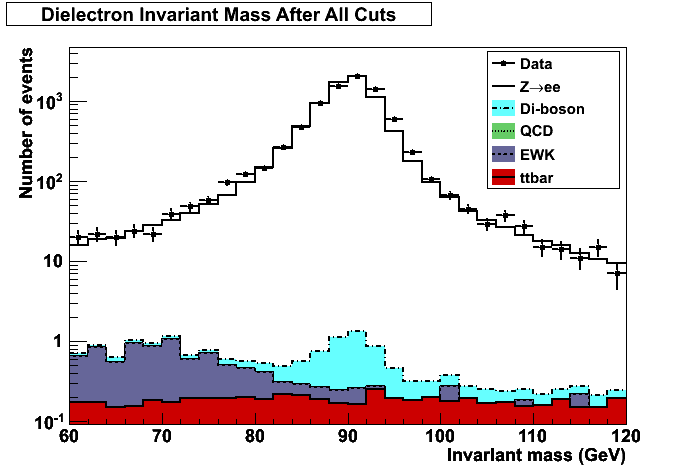
\includegraphics[width=360pt]{Figures/invMass-04Apr11.png}
  \end{center}
  \caption[Electron-pair invariant mass after full selection]
  {Electron-pair invariant mass after full selection.
    The peak around the Z mass (91 GeV) is clearly visible
    in both the Monte Carlo (solid) and data (points) distributions.
    The background contributions estimated from Monte Carlo simulation
    are shown as the colored (grayscale) areas.
    A slight shift in the peak position along the x-axis is
    evident, due to slight miscalibrations of
    the calorimeter response to given energies.
    This difference is accounted for in the
    systematic uncertainty due to the electron energy scale.
  }
  \label{fig:InvMass}
 \end{figure}

% Also add plots for OS and SS??  Had them at one point!  
% WELL, last OS plot I have does not show good data/MC agreement

%% Figures: Same-sign dielectron invariant mass for electrons passing all selection steps, Fig. \ref{fig:SameSignInvMass}

%%  \begin{figure}[htb]
%%   \begin{center}
%%     
\includegraphics[width=360pt]{CMS-BW.pdf}
%%   \end{center}
%%   \caption[Same-sign dielectron invariant mass for electrons passing all selection steps]{Same-sign dielectron invariant mass for electrons passing all selection steps.}
%%   \label{fig:SameSignInvMass}
%%  \end{figure}

%Ooh, I do also have inv mass by eta plots

 \begin{figure}[htb]
  \begin{center}
%    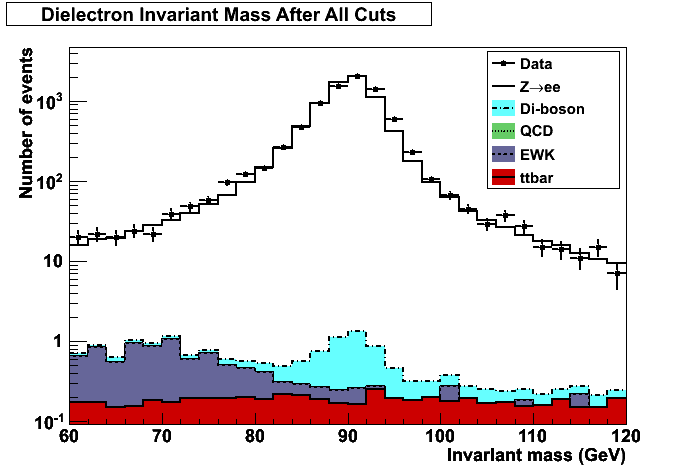
\includegraphics[width=360pt]{Figures/invMass-04Apr11.png}
    \subfloat[Barrel-barrel]{\label{fig:InvMassEtaDivBarrelBarrel}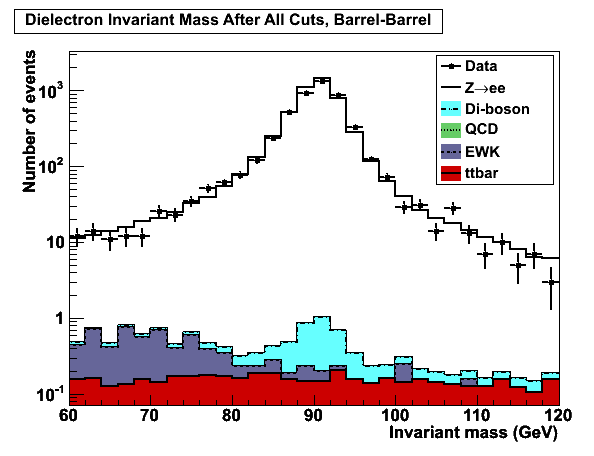
\includegraphics[width=180pt]{Figures/invMassEtaDiv-barrel-barrel-19May11.png}}
    \subfloat[Barrel-endcap]{\label{fig:InvMassEtaDivBarrelEndcap}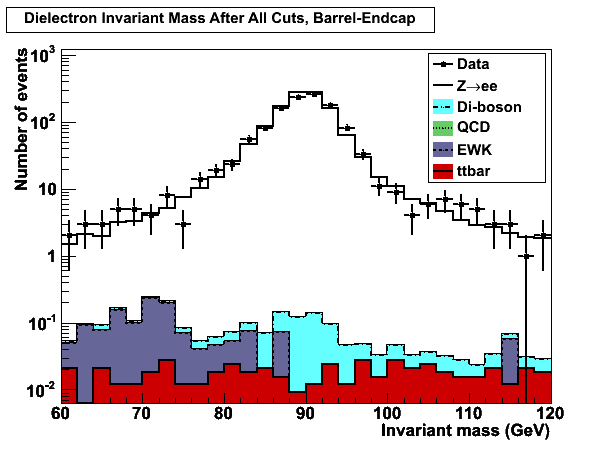
\includegraphics[width=180pt]{Figures/invMassEtaDiv-barrel-endcap-19May11.png}}
    \subfloat[Endcap-endcap]{\label{fig:InvMassEtaDivEndcapEndcap}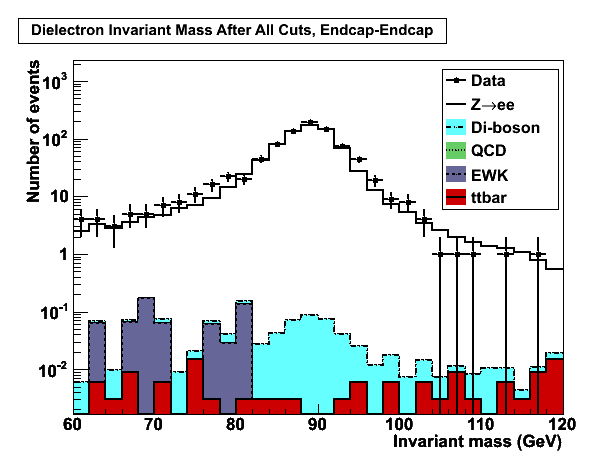
\includegraphics[width=180pt]{Figures/invMassEtaDiv-endcap-endcap-19May11.png}}
  \end{center}
  \caption[Electron-pair invariant mass by $\eta$]{
    Electron-pair invariant mass by $\eta$ after full selection.
    Each combination of electron $\eta$-positions is 
    distributed separately: 
    both electrons in the barrel 
    %(Fig.~\ref{fig:InvMassEtaDivBarrelBarrel}), 
    \subref{fig:InvMassEtaDivBarrelBarrel}, 
    one electron each in the barrel and the endcap 
    %(Fig.~\ref{fig:InvMassEtaDivBarrelEndcap}),
    \subref{fig:InvMassEtaDivBarrelEndcap},
    and both electrons in the endcap 
    %(Fig.~\ref{fig:InvMassEtaDivEndcapEndcap}).
    \subref{fig:InvMassEtaDivEndcapEndcap}.
    In each case the agreement between data and Monte Carlo simulation is good.  
  }
  \label{fig:InvMassEtaDiv}
 \end{figure}

\section{Cross-Section Extraction}
\label{anMeth:xsec}
The formula to calculate the cross section from 
Section~\ref{over:xsec} is
\[
%\sigma_{ Z } \times \textrm{ BR }_{ Zee } = \frac{ n_{ \Zee } }{  \mathcal{ L } \times \epsilon }
\sigma_{ Z } \times \textrm{ BR }_{ Zee } = 
\frac{ n_{signal} }{  \mathcal{ L } \times \epsilon \times A}
\]
where $\mathcal{ L }$ is the luminosity, 
$n_{signal} = n_{total} - n_{background}$ is 
the number of signal events, 
derived from the total number of selected events 
and the estimated number of background events, 
and 
\[
%\epsilon = \epsilon_{ acc } \times \epsilon_{ trig } 
\epsilon = \epsilon_{ reco } \times \epsilon_{ sel } \times \epsilon_{ trig }
\]
is the event selection efficiency, 
composed of the efficiencies of the individual steps: 
%where the abbreviations refer to %acceptance, 
reconstruction, selection, and trigger, respectively.  
%Essentially it means that. %FIXME or just do in overview?
%Most of the required numbers have been dealt with 
%in other chapters.  % remove?
Many of the elements of these formulas have been 
determined in previous sections: 
the event selection efficiency $\epsilon$ was 
calculated as 0.610 
in Section~\ref{evSel:eff}, 
and the acceptance as 0.387 
in Section~\ref{evSel:acc}.  
The luminosity is known to be 36.1 \pb 
(Section~\ref{exp:lumi}). 
The remaining component to be determined 
is the number of signal events, 
which is obtained from the total 
number of selected events 
and the estimated number of background 
events.  
The total number of selected events is 
the number of events in the 
invariant mass histogram, 
Fig.~\ref{fig:InvMass}: 
this is \nevents{} events.  
The final element, estimated number 
of background events, 
will be calculated in 
Section~\ref{anMeth:BGSub}.  


%Explain formula in detail here?  
%It really is the analysis method.  
%You plug in the numbers and get the cross section.  
%Some of the pieces have been done in other 
%chapters, like acceptance and efficiency 
%(ntotal is done above, I guess, just from 
%looking at inv mass plot which isn't strictly 
%necessary, either!)  
%Should they instead all be done here?  

%recap of formula:

%THE FORMULA

%   * ntotal
%   * nbg -- THE DIFFERENT METHODS OF BACKGROUND SUBTRACTION
%   * acc (event sel)
%   * eff (event sel) -- but talk about correcting for data/MC difference
%   * Lumi (exp chapter or sth)

%ntotal comes from inv mass plot just shown, nbg is what you need to calculate.

%The total number of data events surviving 
%the selection cuts is \nevents{}. %8453.  

%3 methods: 
%   * MC estimate
%   * template method
%   * sideband subtraction

%You know, I don't think my analysis needs a whole giant section on data vs MC comparison.  
%I didn't do a whole lot on that.  
%Well, just write up what I did do, I guess.  

%\section{Comparison of Monte Carlo and Data}
\section{Background Subtraction}
\label{anMeth:BGSub}
It is expected that some number of non-signal events %, 
%or background events, 
will look enough like signal events to pass the full selection.  
These background events need to be accounted for 
in the final calculation to arrive 
at the most accurate result.  
Therefore, the number of background events should 
be estimated and subtracted from the total number 
of events; 
this estimation can be done in a variety of ways.  
The methods used in this analysis are detailed 
in the following sections.  

%%% FIXME! MAKE THESE PLOTS???

%% Figures: Background subtracted yield versus eta with a MZ mass window - comparison to MC, Fig. \ref{fig:YieldVsZEtaComparedToMC}

%%  \begin{figure}[htb]
%%   \begin{center}
%%     
\includegraphics[width=360pt]{CMS-BW.pdf}
%%   \end{center}
%%   \caption[Background subtracted yield versus eta with a MZ mass window - comparison to MC]{Background subtracted yield versus eta with a MZ mass window - comparison to MC.}
%%   \label{fig:YieldVsZEtaComparedToMC}
%%  \end{figure}

%% Figures: Background subtracted Z PT distribution with a MZ mass window - comparison to MC, Fig. \ref{fig:YieldVsZPtComparedToMC}

%%  \begin{figure}[htb]
%%   \begin{center}
%%     
\includegraphics[width=360pt]{CMS-BW.pdf}
%%   \end{center}
%%   \caption[Background subtracted Z PT distribution with a MZ mass window - comparison to MC]{Background subtracted Z PT distribution with a MZ mass window - comparison to MC.}
%%   \label{fig:YieldVsZPtComparedToMC}
%%  \end{figure}

\subsection{Monte Carlo Estimation}
\label{anMeth:BGSubMC}
One estimate of the number of background events can be made 
directly from the Monte Carlo simulation, 
by counting the number of simulated events that pass 
the full selection.  
The numbers of passing events for the simulated background 
samples used are shown in Table~\ref{TableBackgroundMC}, 
with a total of 18.5 events.  
The accuracy of this method may be questionable due to 
unaccounted differences between the simulation and real data, however.  
In particular, 
the detector may not be correctly modeled in the simulation, 
causing slight differences in event numbers 
that are non-negligible at this level.  
Therefore, data-driven methods of background subtraction 
are also used, 
and the results from all the methods are checked against each other 
to confirm the accuracy of each method.  

%TABLE with MC-estimated number of events from each background source

\begin{table}[htbp]
%  \centering
  \begin{center}
    \caption{Number of events passing full selection 
      for each background, estimated from 
      Monte Carlo simulation.}
    \label{TableBackgroundMC}
%    \begin{tabular}[]{ | l | c | c | }
    \begin{tabular}[]{ | l | c | }
      \hline
      Background Sample & Number of Events  \\ \hline \hline
      Wenu & 0.36 \\ \hline % 0.35799
      Wtaunu & 0.0 \\ \hline % 0
      Ztautau & 6.4 \\ \hline % 6.3777
      Electroweak Total & 6.7 \\ \hline \hline % 6.73569
      ttbar & 5.8 \\ \hline \hline % 5.83397
      QCD & 0.0 \\ \hline \hline % Hah
      WW & 1.5 \\ \hline % 1.5382
      WZ & 1.4 \\ \hline % 1.4396
      ZZ & 3.0 \\ \hline % 2.9984
      Di-boson Total & 6.0 \\ \hline \hline % 5.9762
      Total Background & 18.5 \\ \hline % 18.54586
    \end{tabular}
  \end{center}
\end{table}



\subsection{Template Method}
\label{anMeth:BGSubTemplate}
The template method is a data-driven method 
to estimate the background contribution 
in a selected sample.  
In general, it uses modified cuts 
to select data events that are especially 
likely to be signal or background; 
these subsamples are called templates.  
Extra-tight cuts select a ``signal-rich'' sample, 
while a combination of loose and inverted cuts 
select a ``background-rich'' sample.  
A particular selection variable is chosen 
which has significantly different distributions 
for signal and background; 
here, the relative tracker isolation variable is used.  
The template method compares the 
distributions of that variable 
from the selected signal and background templates 
to the distribution from the full data sample. %, 
Essentially, the method determines what 
combination of the signal and background templates 
best fits the data distribution, 
in an effort to determine what fraction 
of the data sample is signal 
and what fraction is background.  
This method is only useful to determine the 
background from QCD; 
its technique relies on ``background'' electrons 
being qualitatively different from 
``good electrons'' 
(measured by the variable being used), 
but electrons from interactions similar 
to the signal interaction, 
such as \Wenu, 
are also ``good electrons.''  
Objects arising from QCD interactions that are 
identified as ``electrons'' are more likely 
clusters of hadronic particles 
that come out looking like electrons, 
so they can be distinguished from 
``good electrons'' and therefore 
%used in this method.  
%used for this method.  
the template method can identify 
them as background.  

\subsubsection{Template Definitions}
\label{anMeth:BGSubTemplateDefs}
%defs of tighter and looser selections (bleah), more tables?

Several new working points, based on WP80 
%(defined in Section~\ref{evSel:elec}), 
(see Section~\ref{evSel:elec}), 
were defined to select 
the signal-like and background-like template samples, 
as well as the data distribution used in the comparison.  

The first working point, used to select the data, 
is called ``Semi-Tight'' and is identical to WP80 
except for the removal of its relative track isolation 
requirement.  
This is solely to allow the full spectrum of track 
isolation values to be examined.   
All events with two electrons passing the 
Semi-Tight working point are 
included in the data sample.  

The working point used to select the ``signal-rich'' 
data sample is called ``Tight'' 
and is based on the Semi-Tight working point 
but with a few cuts made tighter.  
(This is to ensure a very pure sample; 
however, a very tight working point would not work 
for standard data selection because its 
efficiency is lower -- 
it cuts out too many good events.  
For the template method, though, a lower number 
of events is sufficient.)  
The tighter cut values were taken from WP70, 
another of the standard working points. %, 
%and the modified values are given in Table~\ref{TableWPs}.  
%In particular, 
Specifically, 
the values for 
\dphiin in both the barrel and the endcap, 
$H/E$ in the barrel, 
and \detain in the endcap 
were modified.  
To select the signal template sample, 
each event was required to have two electrons 
passing the Tight working point, 
and the two electrons were required to have 
opposite signs.  

The final working point used for the template method 
is the ``Loose'' working point, 
which is used in selecting the background template.  
The Loose working point is modeled on the 
Semi-Tight working point, as is the Tight, 
but for the Loose working point 
all the thresholds for the isolation 
and electron isolation variables 
are increased by a factor of 5.  
In addition, in order to get enough data 
for a reasonable background template, 
the ECAL isolation variable had to be further loosened, 
from 0.07 to 2.5 in the barrel and from 0.05 to 1.0 in the endcap, 
and the supercluster \Et cut had to be lowered 
from 25 GeV to 20 GeV.  
Events selected for the background template 
must have two electrons, 
one passing the Semi-Tight working point 
and one passing the Loose, 
and these two electrons are required to 
have the same sign in order to reject signal.  

%HOW TO DO TABLES: just one giant table showing all WP's?  
%highlight changed values?  HA, with italics
%(or tables of just changed values?)

Table~\ref{TableWPs} shows the cut values for 
WP80 and how each of the working points used 
in the template method is modified with 
respect to WP80.  
Cut values changed with respect to WP80 
are displayed in italics.  


% WP'S
\begin{table}[htbp]
%  \centering
  \begin{center}
    \caption{
      Summary of the standard working point as well as 
      the working point definitions used 
      in the template method.
      Italics indicates a cut changed relative to WP80.
    }
    \label{TableWPs}
%    \begin{tabular}[]{ | l | c | c | }
    \begin{tabular}[]{ | l | c | c | c | c | c | c | c | c | }
      \hline
      Cut Variable & \multicolumn{2}{|c|}{WP80} & \multicolumn{2}{|c|}{Semi-Tight} & \multicolumn{2}{|c|}{Tight} & \multicolumn{2}{|c|}{Loose}  \\ \hline \hline
      & Barrel & Endcap & Barrel & Endcap & Barrel & Endcap & Barrel & Endcap \\ \hline
%      Conversion Rejection    & & & & & & & &  \\ \hline % 
      \multicolumn{9}{|l|}{Conversion Rejection}   \\ \hline % 
      missing hits            & 0    & 0    & 0    & 0    & 0    & 0    & 0    & 0     \\ \hline % 
      dist                    & 0.02 & 0.02 & 0.02 & 0.02 & 0.02 & 0.02 & 0.02 & 0.02  \\ \hline % 
      $\delta\cot\theta$      & 0.02 & 0.02 & 0.02 & 0.02 & 0.02 & 0.02 & 0.02 & 0.02  \\ \hline % 
%      Relative Isolation & & & & & & & &  \\ \hline % 
      \multicolumn{9}{|l|}{Relative Isolation}   \\ \hline % 
      ECAL      & 0.07 & 0.05 & 0.07 & 0.05 & 0.07 & 0.05 & \textit{2.5} & \textit{1.0}  \\ \hline % 
      HCAL      & 0.1 & 0.025 & 0.1 & 0.025 & 0.1 & 0.025 & \textit{0.5} & \textit{0.125}  \\ \hline % 
      track     & 0.09 & 0.04 & \textit{N/A} & \textit{N/A} & \textit{N/A} & \textit{N/A} & \textit{N/A} & \textit{N/A}  \\ \hline % 
%      Electron Identification & & & & & & & &  \\ \hline % 
      \multicolumn{9}{|l|}{Electron Identification}   \\ \hline % 
      \sieie          & 0.01  & 0.03  & 0.01  & 0.03  & 0.01  & 0.03  & \textit{0.05} & \textit{0.15}  \\ \hline % 
      \dphiin         & 0.06  & 0.03  & 0.06  & 0.03  & \textit{0.03} & \textit{0.02} & \textit{0.3} & \textit{0.15}  \\ \hline % 
      \detain         & 0.004 & 0.007 & 0.004 & 0.007 & 0.004 & \textit{0.005} & \textit{0.02} & \textit{0.035}  \\ \hline % 
      $H/E$           & 0.04  & 0.025 & 0.04  & 0.025 & \textit{0.025} & 0.025 & \textit{0.2} & \textit{0.125}  \\ \hline % 
      Supercluster \Et & \multicolumn{2}{|c|}{25} & \multicolumn{2}{|c|}{25} & \multicolumn{2}{|c|}{25} & \multicolumn{2}{|c|}{\textit{20}}  \\ \hline % 
    \end{tabular}
  \end{center}
\end{table}

%\textit{italics}

%\subsubsection{TFractionFitter} %need a whole subsection??
%where to mention TFractionFitter itself, and give a little documentation?
%here, I guess
%ALSO NEED A REFERENCE TO TFRACTIONFITTER -- 
%look up the reference on that root page?  
%And/or just give URL of class page as reference?  
%they have some funky stuff to say about statistics and errors...
%AND, also find some way to have reference to the AN??  
%where I got some of this stuff from??

The mechanics of the fit are done by the ROOT class 
TFractionFitter, %.  % easy wy to make fixed-width?
whose purpose is to perform the exact sort of fit 
needed for the template method.  
It determines the composition of 
template distributions that best 
fits a given ``data'' distribution 
using a likelihood fit.  
%In the process, it takes into account 
%uncertainties in both the templates 
%and the data due to statistics.  
Statistical uncertainties in both the 
templates and the data are 
taken into account in the fitting process.  

%http://root.cern.ch/root/html522/TFractionFitter.html  or just ``html'' instead of html522?  
%Is there some kind of permanent class reference??
%paper and stuff: Fits MC fractions to data histogram (a la HMCMLL, see R. Barlow and C. Beeston,
% Comp. Phys. Comm. 77 (1993) 219-228, and http://www.hep.man.ac.uk/~roger/hfrac.f).
%but I don't think that's about TFractionFitter itself.  

\subsubsection{Results}
\label{anMeth:BGSubTemplateResults}
%fit plots -- the signal/background template distribution, as well as full data and fit.  

%Also need to explain plots and results in this section

The relative tracker isolation distributions of the 
signal and background templates are shown in 
Fig.~\ref{fig:TemplateShapes}.  
Each curve independently integrates to 1
and shows the fraction of events of the given type
with relative tracker isolation in each bin.
The difference in shape between signal (solid, black) 
and background (dotted, red)
is clear:
the background has a much higher fraction of events
with higher values of isolation,
while the data has a much higher fraction of events
with lower values.
The lowest bin contains 90\% of signal compared with
around 65\% of background.
These features enable the template method in general 
and the TFractionFitter in particular 
to fit the shape of the templates to the 
distribution of the data.  
The data distribution is shown in 
Fig.~\ref{fig:TFractionFit} 
as the hollow circles (black), 
while the fit as determined by the
TFractionFitter is displayed as asterisks (red).  
The agreement is very good, showing that 
TFractionFitter was able to make a good 
match between the data and its combination 
of templates.  

 \begin{figure}[htb]
  \begin{center}
%    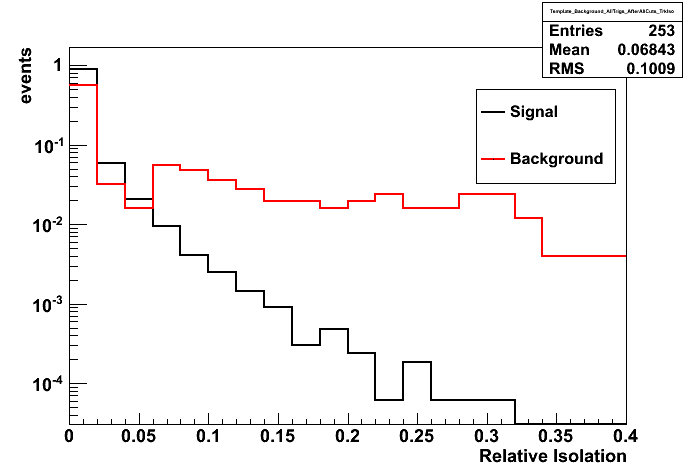
\includegraphics[width=360pt]{Figures/TemplateShapes-01Mar11.png}
    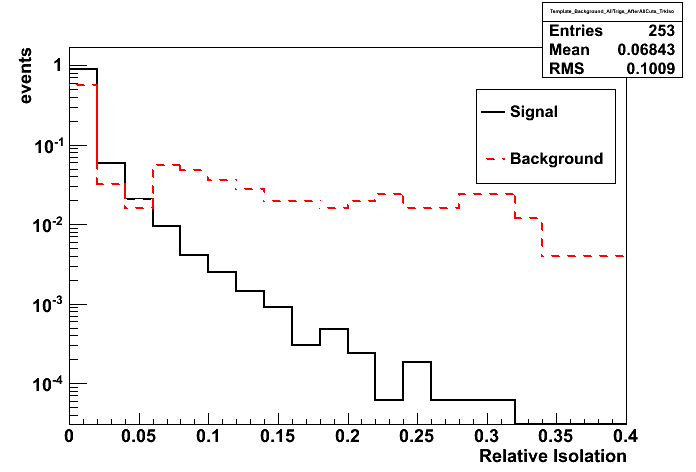
\includegraphics[width=360pt]{Figures/TemplateShapes-01Mar11-lines.png}
  \end{center}
  \caption[Shapes of signal and background templates used in 
    template method of background subtraction]{
    Shapes of signal and background templates 
    used in template method of background subtraction.
    Each curve independently integrates to 1 
    and shows the fraction of events of the given type 
    with relative tracker isolation in each bin.  
    The solid (black) curve represents signal 
    and the dotted (red) shows background.  
    The difference in shape between the two categories 
    is clear: 
    the background has a much higher fraction of events 
    with higher values of isolation, 
    while the data has a much higher fraction of events 
    with lower values.  
    The lowest bin contains 90\% of signal compared with 
    around 65\% of background.  
    This difference is exploited 
    in the template method 
    to determine the 
    signal vs. background composition of a given 
    data sample.  
  }
  \label{fig:TemplateShapes}
 \end{figure}

 \begin{figure}[htb]
  \begin{center}
    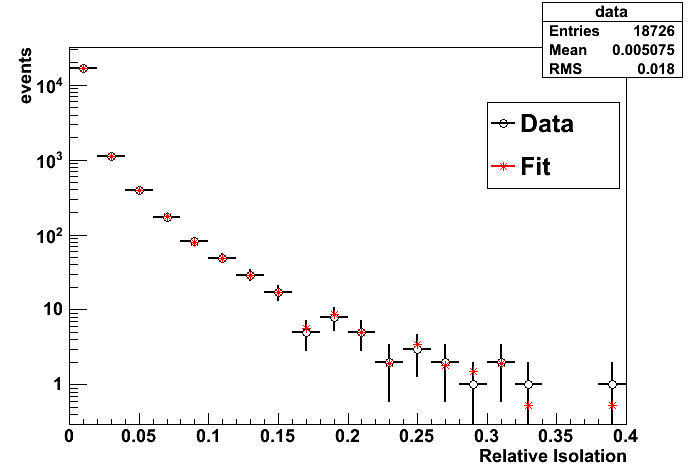
\includegraphics[width=360pt]{Figures/TFractionFitter-full-01Mar11.png}
  \end{center}
  \caption[Results of template fit to data]{
    Results of template fit to data.
    The relative track isolation distribution 
    for the data sample 
    is shown as the hollow circles (black), 
    while the TFractionFitter-determined 
    template fit, 
    using a combination of the signal 
    and background templates, 
    is shown as the asterisks (red).  
    The fit agrees very well to the data; 
    small deviations are visible but 
    are contained within the data error bars.  
  }
  \label{fig:TFractionFit}
 \end{figure}

Over the full range of the relative tracker isolation 
values used for the template fit, 
the fraction of signal was determined to be 
0.998 +/- 0.014, 
while the fraction of background was calculated to be 
0.0016 +/- 0.0020.  
However, the signal fraction over the full 
range is not useful, because this includes 
background events that would fail 
the tracker isolation selection cut.  
Therefore, the tracker isolation cut is effectively 
reapplied by only looking at events which 
pass the cut.  
In effect this is done by integrating 
the number of signal and background events 
below the threshold and redetermining the 
signal and background fractions.  
%This is done with the following formula: 
This is represented in the formula 
\[
f_{sig}^{thresh} = \frac{ f_{sig} \times n_{sig}^{thresh} }{ f_{sig} \times n_{sig}^{thresh} + f_{bg} \times n_{bg}^{thresh} }
\]
which in essence scales the signal fraction 
according to the relative number of events 
below the threshold.  
In this case $f_{sig}$ and $f_{bg}$ are the 
signal and background fractions determined 
from the full isolation spectrum, 
while $f_{sig}^{thresh}$ is the signal fraction 
below the isolation threshold.  
$n_{sig}^{thresh}$ and $n_{bg}^{thresh}$ are the 
integrated signal and background event numbers 
below the threshold.  
Since the barrel and endcap thresholds 
for relative tracker isolation are different, 
the integration and fraction 
redetermination was performed with each 
threshold separately.  
However, the differences in the final fractions 
were negligible (non-existent within significant figures), 
so using the barrel threshold vs. the endcap threshold 
was determined not to be a significant factor.  
The signal fraction below the threshold was determined 
to be 1.000 +/- 0.014, and the background fraction 
0.000 +/- 0.002.  
It is expected that the background fraction below 
the cut threshold would be lower than over the 
entire spectrum, 
since more of the background distribution 
was above the cut threshold than the data distribution.  
The calculated values therefore agree with the 
expectation in that sense.  

The signal and background fractions of the data sample 
determined both from the full isolation spectrum and 
from the spectrum below the cut threshold are shown in 
Table~\ref{TableSignalBGFractions}.  

\begin{table}[htbp]
  \begin{center}
    \caption[Signal and background fractions of data sample]{
      Signal and background fractions of data sample, 
      for both the full relative tracker isolation 
      spectrum and for the part of the spectrum 
      below the cut threshold.  
    }
    \label{TableSignalBGFractions}
    \begin{tabular}[]{ | l | c | c | }
      \hline
      & Full spectrum & Below threshold  \\ \hline \hline
      Signal fraction & 0.998 +/- 0.014 & 1.000 +/- 0.014 \\ \hline 
      Background fraction & 0.0016 +/- 0.0020 & 0.000 +/- 0.002 \\ \hline
    \end{tabular}
  \end{center}
\end{table}

The background fraction for the data sample measured 
below the isolation cut threshold 
translates to a event count of 0 +/- 16.8 events.  
(It should be recalled that this method is only 
considered valid for estimating QCD background.)  
The relative uncertainty on the number of signal 
events corresponding to the error (16.8 events) 
is 0.2\%.  % RELATIVE UNCERTAINTY NOT DEFINED YET
% maybe move that bit to uncertainty section, 
% to have it all together?  


\subsection{Sideband Subtraction}
\label{anMeth:BGSubSideband}

An additional method of estimating background was 
attempted, to cross-check the other two.  
This method involved fitting the invariant mass 
peak with a lineshape to model the signal plus 
one to model the background, 
in the standard sideband subtraction method.  
This is similar to the template method used in 
the previous section, 
in that a distribution is fitted to a composition 
of signal and background contributions.  
However, the sideband subtraction method 
uses a different variable distribution, 
the invariant mass peak, 
as well as a different set of components 
with which to fit the distribution.  
Getting the same results with such 
different methods adds strength to 
the claim that the results are accurate.  
The name ``sideband subtraction'' refers 
to taking the distribution in 
the areas away from the peak, the ``sidebands'', 
to represent the background part of the contribution, 
%and 
extrapolating it into the peak area, and 
subtracting it from the total distribution 
to leave only the signal contribution.  

% FIXME
%explanations of what gozinta fits 
%(how much did I explain 
%about lineshapes in tag and probe?)

The data invariant mass spectrum is fitted with 
the same lineshapes used to determine the efficiency 
with the tag-and-probe method (see Section~\ref{evSel:eff}).  
That is, the data is fit with the \Zee spectrum 
shape taken from the generator-level, 
convolved with a Crystal Ball function 
times a Gaussian function, 
which represents the signal, 
while using an exponential function to represent 
the background.
% FIXME EXPLAIN ALL THESE FUNCTIONS SOMEWHERE
The resulting fit is shown in Fig.~\ref{fig:ZFit}.  
Fig.~\ref{fig:ZFitLin} shows the fit in linear
scale, while Fig.~\ref{fig:ZFitLog} shows the
same plot in logarithmic scale.
The total composition of lineshapes is shown as the
solid line.
The background contribution is shown as a dotted line,
and is only visible in Fig.~\ref{fig:ZFitLin}, the
linear-scale plot.
In logarithmic scale the exponential contribution is
drawn around $10^{-3}$ and hence is not displayed
on the logarithmic-scale plot.


%plots of fit
 \begin{figure}[htb]
  \begin{center}
%    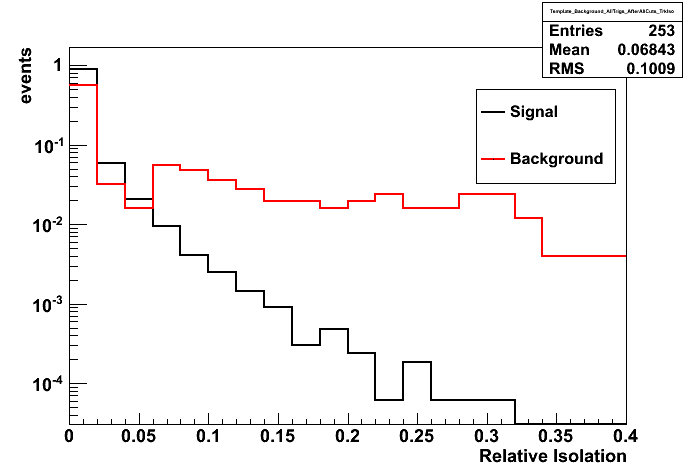
\includegraphics[width=360pt]{Figures/TemplateShapes-01Mar11.png}
%    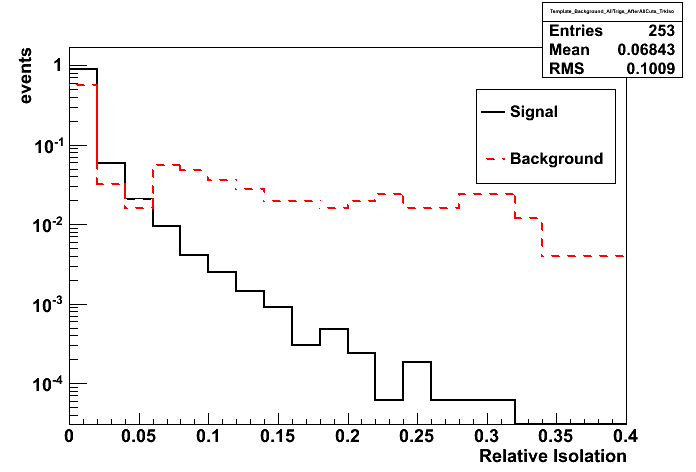
\includegraphics[width=360pt]{Figures/TemplateShapes-01Mar11-lines.png}
    \subfloat[Linear scale]{\label{fig:ZFitLin}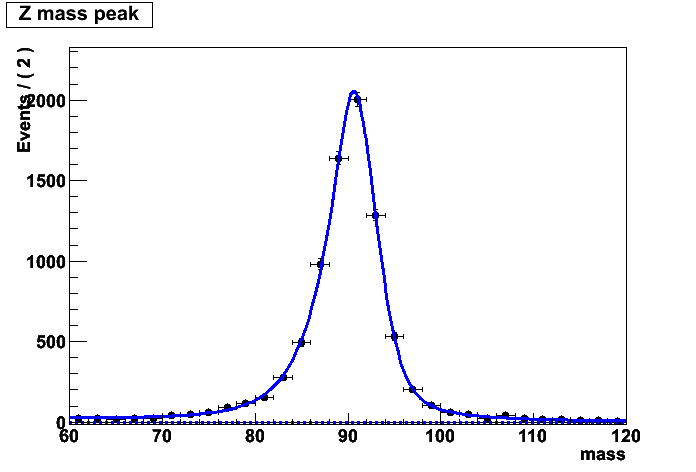
\includegraphics[width=180pt]{Figures/ZFit-lin-08Mar11.png}}
    \subfloat[Logarithmic scale]{\label{fig:ZFitLog}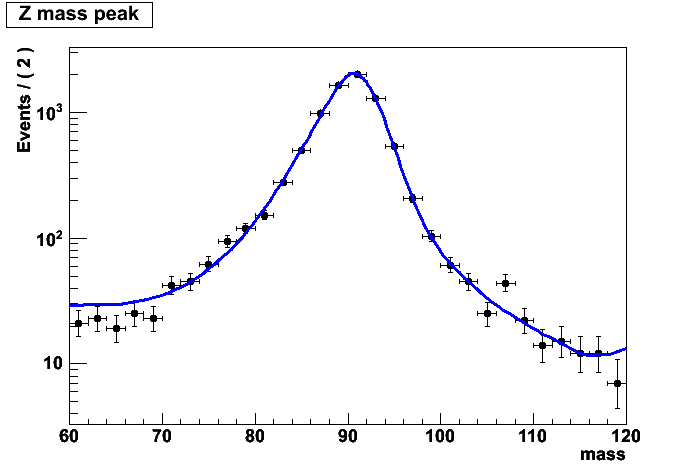
\includegraphics[width=180pt]{Figures/ZFit-log-08Mar11.png}}
  \end{center}
  \caption[Functional fit of \Zee invariant mass peak 
    for background subtraction]{
    Fit of \Zee invariant mass peak for the purpose 
    of background subtraction.  
    %Fig.~\ref{fig:ZFitLin} 
    \subref{fig:ZFitLin} 
    shows the fit in linear 
    scale, while 
    %Fig.~\ref{fig:ZFitLog} 
    Fig.~\subref{fig:ZFitLog} 
    shows the 
    same plot in logarithmic scale.  
    The peak is fit with a combination of 
    lineshapes representing the signal, 
    the generator-level lineshape convolved with 
    a Crystal Ball function convolved with a Gaussian, 
    and a Gaussian lineshape representing the background.  
    The total composition of lineshapes is shown as the 
    solid line.  
    The background contribution is shown as a dotted line, 
    and is only visible in 
    %Fig.~\ref{fig:ZFitLin}, 
    \subref{fig:ZFitLin}, 
    the linear-scale plot.  
    In logarithmic scale the exponential contribution is
    drawn around $10^{-3}$ on the vertical scale 
    and hence is not displayed 
    on the logarithmic-scale plot.  
  }
  \label{fig:ZFit}
 \end{figure}

%results/numbers/discussion of random little things

In general it appears that the agreement of the fit 
with the actual data points is quite good.  
However, there are certain features of the fit 
that bear explaining.  
In particular, 
at the lower and upper tails of the peak, 
the fit appears to be higher than the data points, 
and at the upper end an ``uptick'' in the fit 
curve appears.  
This is due to statistical fluctuations in 
the generator-level \Zee spectrum histogram.  
That histogram is very finely binned, 
and small fluctuations affect the shape of the final fit.  
The discrepancy at the lower end is likewise 
due to the shape of the generator-level histogram.  
The contribution of the background function to the 
overall fit is negligible.  
%what about the shoulder and the bump at 108?
In addition, there appears to be a ``shoulder'' 
in the data points between about 75 and 80 GeV, 
as well as a fluctuation around 108 GeV.  
At this point in time these features in the shape 
are not understood but have been seen in 
other analyses as well.  %REFERENCE??
However, since they involve relatively few events, 
and because the analysis does not largely 
depend on the shape of the spectrum, 
for this analysis they can be ignored.  

The composition of signal and background 
functions to the overall lineshape 
gives the number of background events 
to be 0 +/- 14 events.  


\subsection{Comparison of Background Subtraction Methods}
\label{anMeth:BGSubComp}
%Do overall analysis of comparison of background subtraction methods
%in its own section

The three methods of background estimation 
detailed in the previous sections have yielded 
roughly consistent results, 
summarized in Table~\ref{TableBGSub}.  
It is interesting that both of the methods 
that looked at data arrived at a total 
of 0 background events.  
The template method only gives an estimate for 
QCD events, 
but the estimate from invariant mass fit 
applies to all sources of background.  
These values of zero inherently look suspicious; 
a value of 0 anywhere in a fit 
means that something 
has hit its limit in the optimization 
algorithm.  
However, investigations into the two methods 
have yielded nothing inherently faulty.  
With the template method in particular 
it took many iterations of the criteria 
to obtain a ``background-like'' sample 
large enough to work with, 
supporting the idea that the selection 
cuts are very effective at eliminating background.  
In addition, more than one independent 
method of analysis is giving the same result.  
Furthermore, the errors on both of those numbers 
are approximately the value of the background 
predicted by Monte Carlo simulation.  
Therefore, the actual background number 
could be 0 or 19 or somewhere in between 
and still be basically consistent with 
all three methods.  
For the purposes of this analysis, 
the most conservative values obtained 
with any of the three methods were 
taken for both the estimated number 
of background events and the error estimate.  
This yielded a background estimate of 
19 events from the Monte Carlo estimate, 
and an error of 17 events from the template method.  

\begin{table}[htbp]
  \begin{center}
    \caption[Summary of background estimates from different methods]{
      Summary of background estimates from the three 
      different methods used in this analysis.  
      All three methods give roughly consistent results.  
      In general the most conservative values have been used.  
    }
    \label{TableBGSub}
    \begin{tabular}[]{ | l | c | c | }
      \hline
      Method & Background events & Error (events)  \\ \hline \hline
      Monte Carlo & 18.5 & N/A \\ \hline 
      Template Method & 0 & 16.8 \\ \hline 
      Sideband Subtraction & 0 & 14 \\ \hline 
    \end{tabular}
  \end{center}
\end{table}


\section{Estimation of Systematic Uncertainties}
\label{anMeth:Systs}
%MAYBE MAKE WHOLE OTHER CHAPTER???

% SOME TEXT HERE???

\subsection{Introduction to Error Analysis}
\label{anMeth:SystsIntro}

When making any sort of measurement it is essential 
to know how accurate the result is.  
This accuracy can be quantified in the 
``error'' or ``uncertainty'' 
on a measurement, 
meaning the bounds around the measured value 
within which the true value can be assumed to lie.  
A measurement with a smaller error is 
therefore a more accurate or ``better'' result, 
and hence calculating the error on a result is 
an extremely important part of 
any analysis.  

An uncertainty on a quantity can be 
expressed in two different ways.  
The first way is as an absolute uncertainty, 
with the same units as the quantity, 
for example ``20.0 +/- 0.2 grams''.  
The second way is as an uncertainty 
relative to the value of the quantity itself, 
such as ``20.0 grams +/- 1\%''.  
The ``1\%'' comes from the value of the absolute 
uncertainty divided by the value of the quantity: 
%$0.2 grams/20.0 grams = 0.01 = 1\%$. 
0.2 grams/20.0 grams = 0.01 = 1\%. 
The relative uncertainty is therefore unitless.  

%ADDING ERRORS IN QUADRATURE

In order to combine the effects of 
different (independent) uncertainties, 
it is necessary to add them 
in quadrature, as shown:
\[
\left(\frac{\delta X_{tot}}{X_{tot}}\right)^2 
= \sum_{i=1}^{N} \left(\frac{\delta X_i}{X_i}\right)^2 
= \left(\frac{\delta X_1}{X_1}\right)^2 
+ \left(\frac{\delta X_2}{X_2}\right)^2 
+ \ldots
+ \left(\frac{\delta X_N}{X_N}\right)^2 
\]
where 
$X$ is the value of the given quantity and 
$\delta X$ is the absolute error, 
making $\frac{\delta X}{X}$ the relative error.  
Here, $tot$ denotes the total uncertainty 
and $i=1,2,\ldots ,N$ the uncertainties from 
individual sources.  
Only the relative uncertainties 
can be combined in this way, 
due to the lack of different units.  
This formula may be understood 
conceptually by analogy to the 
x-y coordinate plane, in particular 
the formula for a given point's distance 
to the origin.  
%The x and y coordinates of the point 
%are independent of each other
In the same way the square of the total distance 
from zero is given as the sum of the squares 
of the (independent) component distances, 
the square of the ``total uncertainty'' 
is given by the sum of the squares of the 
individual (independent) component uncertainties.  
Instead of calculating a distance in %x-y 
coordinate space, 
this distance is calculated in 
``uncertainty space''.
%For this formula to be true, 
%all sources of uncertainty 
%must be independent.  

In high energy physics the sources of uncertainty 
are generally divided into two categories: 
statistical and systematic.  
Statistical error arises from the fluctuations 
possible when counting elements in a population.  
The higher the number of elements used 
in the study, 
the more accurate the measurement is likely to be.  
%READ MORE ON STATISTICS!!!
In a high energy physics analysis 
this corresponds to the number of events used.  
%FIXME SAY MORE ON THE WHY HERE 
The relative statistical error on a measurement 
is equal to the square root of the total number 
of events divided by the total number of events:
\[
\frac{\delta{}x}{x} = \frac{\sqrt{N}}{N}
\]
Where $x$ is the quantity being measured and 
$N$ is the total number of events used.  
In our case, the statistical error on the final 
result is given by 
\[
%\frac{\sqrt{8453}}{8453}
\frac{\sqrt{\nevents{}}}{\nevents{}} = 1.1\% % sqrt(8453)/8453 = 0.0108766
\]
The statistical error is fixed for a given number 
of events; 
the only way to reduce the statistical error 
is to analyze more events.  

The second type of error, systematic error, 
encompasses everything else that may 
inadvertently 
%change 
affect the result of the analysis.  
The particular sources are specific to the analysis 
in question, 
ranging from slight differences 
in theoretical predictions, 
reflecting our incomplete knowledge of the subject, 
to possible miscalibrations of the detector, 
to possible biases inherent in reconstruction 
or identification algorithms.  
The error is evaluated by changing something 
in the analysis and seeing how much the 
result itself would change.  
Some changes have very little effect, 
while some have larger effects.  
In general, it is only necessary to account 
for the larger effects, 
``larger'' being defined by the scale 
of the statistical uncertainty.  
If the systematic error due to a particular 
source is much smaller than the 
overall statistical error, 
its contribution to the total uncertainty 
is relatively very small, 
and it can safely be ignored.  
It is therefore standard to try to adjust 
an analysis if necessary such that its 
systematic error is at most about the same as 
the statistical error.  
Such corrections might include using 
a reconstruction method whose errors 
are shown to be lower, 
or doing a more thorough analysis 
in which case some errors can be reduced.  


%Woohoo, the whole thing

%   * stat (but that's not syst) -- should just go at end, I guess?  
%OR, make a separate little section to explain the statistical stuff

\subsection{Systematic Uncertainty due to Luminosity}
\label{anMeth:SystsLumi}

%   * lumi

As one of the necessary components in the 
cross-section calculation, 
any uncertainty on the measurement of the luminosity 
is relevant to the final result.  
The luminosity is measured by the forward hadronic calorimeter (HF) 
as explained in Section~\ref{exp:lumi}.  
For the 2010 dataset, 
the luminosity measurement has an accepted 
relative uncertainty value of 4\%.  % REFERENCE

\subsection{Systematic Uncertainties from Theory}
\label{anMeth:SystsTheory}

%   * theory systs (HOW TO REFERENCE??  Just reference VBTF paper, I guess...?)
% the VBTF public paper aka PAS only has 3 lines on the theoretical uncertainties, 
% plus the two entries in the table.  
% I guess I can put in a little more detail, since it's not like it's secret

%intro theory uncertainties

Uncertainties in theoretical predictions do not 
necessarily play a role in an experimental measurement.  
However, the theoretical models do affect the 
calculation of the acceptance (see Section~\ref{evSel:acc}).  
The acceptance must inherently be obtained from 
Monte Carlo simulation, making it dependent on the 
individual model used.  
% how exactly does PDF affect Z rapidity, for example?
Since there are many different possible corrections 
to the given Monte Carlo modeling, 
all of these variations should be taken into account.  
The official CMS \Zee analysis calculated % reference EWK-10-005 pas
uncertainties in the acceptance due to 
various elements of theory, 
and these are given here.  


%details on what they did -- outline of AN 2010/055, basically!

%QCD resummation and NNLO corrections % LOOKUP resummation

The Monte Carlo simulated data sample used in the analysis 
does not include corrections from resummation or 
NNLO QCD corrections.  
There are tools that account for these corrections, 
however, 
namely the ResBos event generator, % REFERENCE
so this generator was used to 
calculate the uncertainty due to the missing corrections.  


%higher order (>NNLO) QCD corrections

Since calculations are generally done up to a fixed order 
and depend on the renormalization and factorization scales, % LOOKUP
varying these scales can estimate the uncertainty due 
to the missing higher-order calculations.  
The scales were therefore varied each way by a factor of two 
and the maximum difference in results was taken, 
using FEWZ to calculate the cross section.  % ADD FEWZ THING TO SIM CH


%PDF -- put to front, in its own section -- others all in same section?

There are several well-known
parton distribution function (PDF) sets
in existence,
and the output of simulations
using these PDFs vary slightly from one another.
Three different PDF sets were used: 
CT10, MSTW2008, and NNPDF2.0.  
The value of the acceptance with each PDF was calculated 
in order to determine the spread between the three sets.  
In addition, the error function corresponding to each PDF 
was evaluated, 
and these were combined with the acceptance spread 
over the PDFs.  
% 0.81\% according to table, 0.9\% according to PAS


%NLO EWK corrections (missing full EWK, uncertainty in FSR; ISR found to be insignificant)

The Monte Carlo simulation sample used for the analysis 
also does not fully account for next-to-leading-order (NLO) 
electroweak corrections.  
In addition, the existing corrections, 
namely final-state radiation, 
may not be completely accurate.  
To deal with these sources of uncertainty, 
a separate generator, HORACE, 
was used to make the full set of corrections.  
The output was then compared with the 
standard simulation sample to estimate 
the uncertainty due to the missing corrections.  

% WHY NOT JUST USE THESE BETTER GENERATORS FOR FULL SAMPLE IN THE FIRST PLACE???

%Guess I'd better give numbers in public note:
%PDF by themselves, others together,
%then combined number

The uncertainty due to the PDF set used 
was found to be 0.9\%, 
while the rest of the sources 
contributed a total of 1.4\%, 
for a combined value of 1.7\% relative uncertainty.  

% WILL BE REVISITED ONCE I'VE LEARNED MORE ABOUT EVENT GENERATORS AND THEORY!




\subsection{Other Sources of Systematic Uncertainty}
\label{anMeth:SystsOther}

%my stuff: 

In addition to the analysis-independent 
uncertainty due to luminosity, 
and the uncertainty in the acceptance 
from the theoretical modeling, 
there are several sources of 
uncertainty specific to this analysis 
that also need to be accounted for.  

\subsubsection{Electron Energy Scale}
\label{anMeth:SystsOtherEleEScale}

%   * electron energy scale

A typical source of systematic uncertainty 
is the energy scale of the physics objects 
used in the analysis, 
depending on the type of physics object.  
The electron energy scale is determined 
by the accuracy of the electromagnetic 
calorimeter (see Section~\ref{exp:ECAL})
at measuring the energy 
deposited by the particles passing into it.  
The response of the ECAL is measured 
using a test beam setup: 
particle beams of known energies are 
directed at the calorimeter material, 
and the response is recorded.  
This response is then correlated with the 
original particle energies.  
% ADD SOMETHING ABOUT THAT TO EXPERIMENT CHAPTER???
% SOME REFERENCE TO TEST BEAM TESTS?
However, the correlation may not be completely 
accurate.  
Scaling the electron energy by an amount 
slightly less than or greater than 1 
and then observing the resulting change 
in the number of \Zee events 
gives an estimate of the systematic error 
due to the electron energy scale.  
Uncertainties of 2\% and 3\% % do I need a reference?  not public,
%it was on HN:
% https://hypernews.cern.ch/HyperNews/CMS/get/egamma/911/1/1/1.html
% https://hypernews.cern.ch/HyperNews/CMS/get/egamma/911/1/1/2.html
for the ECAL barrel and endcap respectively 
were given as conservative values.  
The electrons' energy were then multiplied 
by 1.02 or 1.03 for the upper-end calculation, 
and 0.98 or 0.97 for the lower-end calculation, 
according to their position (barrel or endcap).  
Scaling the energy up resulted in finding 
%67 more \Zee candidate events, 
%for a relative change of 0.82\%.  
%a relative change in number of candidate events 
%of +0.82\%.  
0.82\% more \Zee candidate events.  
On the other hand, scaling the energy down 
%caused the loss of 88 events, 
%for a relative difference of 1.07\%.  
caused the loss of 1.07\% of the events.  
These two changes were averaged 
to give an overall relative error 
of 0.95\% for the final result.  

\subsubsection{Monte Carlo Sample for Efficiency}
\label{anMeth:SystsOtherMCEff}

%   * MC sample for efficiency

As discussed in Chapter~\ref{sim}, 
any given Monte Carlo simulation 
does not necessarily give a completely accurate 
model of particle interactions.  %and their after-effects, decays...?
Therefore, since part of the efficiency calculation 
was based on Monte Carlo simulation samples, 
it is quite possible that the numbers 
derived from simulation are not fully 
accurate.  
This must be accounted for as a systematic 
uncertainty.  
This accounting is done by 
redoing the calculation using samples 
from different Monte Carlo generators.  
In addition to the standard POWHEG generator 
sample, 
two samples generated by PYTHIA were used, 
Tune Z2 and Tune D6T.  
% Table of sample information??
The ``Monte Carlo true'' and ``Monte Carlo tag and probe'' 
efficiencies were evaluated with each sample.  
The difference was quantified by taking the 
maximum spread between the values for each of the 
three samples 
and dividing that number by 2.  
%Indeed, the simulation efficiency 
%varied with the samples used.  
The maximum difference in efficiency occurred 
between the POWHEG and PYTHIA D6T samples, 
with a difference of 2.37\%.  
The total relative systematic uncertainty that can be 
attributed to variation in the Monte Carlo 
sample is therefore 1.19\%.  

% Table with breakdown?  

%This is due to the fact that the simulation 
%programs represent our ``best guess'' 
%as to how the interactions work.  
%They have been shown to generally represent 
%the real interactions fairly well, 
%but small differences exist.  

\subsubsection{Fitting for Efficiency}
\label{anMeth:SystsOtherFitEff}

%   * efficiency fitting

The efficiency calculations in Section~\ref{evSel:eff} 
had associated systematic errors due to the 
goodness of the fit, 
which are the errors shown in Table~\ref{TableEfficiencies}.  
The error on the final event selection 
efficiency is 0.0047 in terms of absolute error, 
or 0.76\% relative error.  


\subsubsection{Background Subtraction/Modeling}
\label{anMeth:SystsOtherBGSub}

%   * background subtraction/modeling (variation among the methods)

As described in Section~\ref{anMeth:BGSubComp}, 
the uncertainty on the number of background 
events was taken to be 17 events, 
from the template method.  
This produces a relative uncertainty 
on the number of signal events 
(and hence final cross section) 
of 0.2\%.  

\subsection{Summary of Uncertainties}
\label{anMeth:SystsSummary}

A summary of the uncertainties on the final 
cross section resulting from various sources 
is shown in Table~\ref{TableSystsSummary}.  
The luminosity contributes 4\% of uncertainty, 
statistics 1.1\%, 
theoretical systematics 1.7\%, 
and experimental systematics a total of 1.7\%.  
% combined theory and exp systs number? 

\begin{table}[htbp]
  \begin{center}
    \caption[Summary of uncertainties]{
      Summary of relative uncertainties from sources 
      including luminosity, theoretical uncertainties, 
      and experimental uncertainties.  
    }
    \label{TableSystsSummary}
    \begin{tabular}[]{ | l | l | }
      \hline
      Source & Value  \\ \hline \hline
      Luminosity Uncertainty & 4\% \\ \hline 
      Statistical Uncertainty & 1.1\% \\ \hline 
      Theoretical Systematics & 1.7\% \\ \hline \hline 
      Experimental Systematics & 1.7\% \\ \hline \hline 
      Electron Energy Scale & 0.95\% \\ \hline 
      MC Sample for Efficiency & 1.2\% \\ \hline 
      Efficiency Fitting & 0.76\% \\ \hline 
      Background Subtraction/Modeling & 0.2\% \\ \hline 
    \end{tabular}
  \end{center}
\end{table}


%\section{What Else?}
%\label{anMeth:WhatElse}
%Is this supposed to be random collection of methods used?  
%e.g. tag and probe, template method, sideband fitting... 
%although I guess the last two are actually background subtraction, 
%which is somehow already determined to be part of this chapter.  
%And Tag and probe is already part of event selection chapter, 
%when talking about event selection efficiency.  